%%
%% Copyright 2007, 2008, 2009 Elsevier Ltd
%%
%% This file is part of the 'Elsarticle Bundle'.
%% ---------------------------------------------
%%
%% It may be distributed under the conditions of the LaTeX Project Public
%% License, either version 1.2 of this license or (at your option) any
%% later version.  The latest version of this license is in
%%    http://www.latex-project.org/lppl.txt
%% and version 1.2 or later is part of all distributions of LaTeX
%% version 1999/12/01 or later.
%%
%% The list of all files belonging to the 'Elsarticle Bundle' is
%% given in the file `manifest.txt'.
%%
\documentclass[5p,,preprint,12pt,twocolumn]{elsarticle}
\makeatletter\if@twocolumn\PassOptionsToPackage{switch}{lineno}\else\fi\makeatother

\usepackage[left]{lineno}
\linenumbers

\usepackage{tabulary,xcolor}
\usepackage{amsfonts,amsmath,amssymb}
\usepackage[T1]{fontenc}
\makeatletter
\let\save@ps@pprintTitle\ps@pprintTitle
\def\ps@pprintTitle{\save@ps@pprintTitle\gdef\@oddfoot{\footnotesize\itshape \null\hfill\today}}
\def\hlinewd#1{%
  \noalign{\ifnum0=`}\fi\hrule \@height #1%
  \futurelet\reserved@a\@xhline}
\def\tbltoprule{\hlinewd{.8pt}\\[-12pt]}
\def\tblbottomrule{\noalign{\vspace*{6pt}}\hline\noalign{\vspace*{2pt}}}
\def\tblmidrule{\noalign{\vspace*{6pt}}\hline\noalign{\vspace*{2pt}}}
\AtBeginDocument{\ifNAT@numbers \biboptions{sort&compress}\fi}
\makeatother

  


\usepackage{ifluatex}
\ifluatex
\usepackage{fontspec}
\defaultfontfeatures{Ligatures=TeX}
\usepackage[]{unicode-math}
\unimathsetup{math-style=TeX}
\else 
\usepackage[utf8]{inputenc}
\fi 
\ifluatex\else\usepackage{stmaryrd}\fi

  
%%%%%%%%%%%%%%%%%%%%%%%%%%%%%%%%%%%%%%%%%%%%%%%%%%%%%%%%%%%%%%%%%%%%%%%%%%
% Following additional macros are required to function some 
% functions which are not available in the class used.
%%%%%%%%%%%%%%%%%%%%%%%%%%%%%%%%%%%%%%%%%%%%%%%%%%%%%%%%%%%%%%%%%%%%%%%%%%
\usepackage{url,multirow,morefloats,floatflt,cancel,tfrupee}
\makeatletter


\AtBeginDocument{\@ifpackageloaded{textcomp}{}{\usepackage{textcomp}}}
\makeatother
\usepackage{colortbl}
\usepackage{xcolor}
\usepackage{pifont}
\usepackage[nointegrals]{wasysym}
\urlstyle{rm}
\makeatletter

%%%For Table column width calculation.
\def\mcWidth#1{\csname TY@F#1\endcsname+\tabcolsep}

%%Hacking center and right align for table
\def\cAlignHack{\rightskip\@flushglue\leftskip\@flushglue\parindent\z@\parfillskip\z@skip}
\def\rAlignHack{\rightskip\z@skip\leftskip\@flushglue \parindent\z@\parfillskip\z@skip}

%Etal definition in references
\@ifundefined{etal}{\def\etal{\textit{et~al}}}{}


%\if@twocolumn\usepackage{dblfloatfix}\fi
\usepackage{ifxetex}
\ifxetex\else\if@twocolumn\@ifpackageloaded{stfloats}{}{\usepackage{dblfloatfix}}\fi\fi

\AtBeginDocument{
\expandafter\ifx\csname eqalign\endcsname\relax
\def\eqalign#1{\null\vcenter{\def\\{\cr}\openup\jot\m@th
  \ialign{\strut$\displaystyle{##}$\hfil&$\displaystyle{{}##}$\hfil
      \crcr#1\crcr}}\,}
\fi
}

%For fixing hardfail when unicode letters appear inside table with endfloat
\AtBeginDocument{%
  \@ifpackageloaded{endfloat}%
   {\renewcommand\efloat@iwrite[1]{\immediate\expandafter\protected@write\csname efloat@post#1\endcsname{}}}{\newif\ifefloat@tables}%
}%

\def\BreakURLText#1{\@tfor\brk@tempa:=#1\do{\brk@tempa\hskip0pt}}
\let\lt=<
\let\gt=>
\def\processVert{\ifmmode|\else\textbar\fi}
\let\processvert\processVert

\@ifundefined{subparagraph}{
\def\subparagraph{\@startsection{paragraph}{5}{2\parindent}{0ex plus 0.1ex minus 0.1ex}%
{0ex}{\normalfont\small\itshape}}%
}{}

% These are now gobbled, so won't appear in the PDF.
\newcommand\role[1]{\unskip}
\newcommand\aucollab[1]{\unskip}
  
\@ifundefined{tsGraphicsScaleX}{\gdef\tsGraphicsScaleX{1}}{}
\@ifundefined{tsGraphicsScaleY}{\gdef\tsGraphicsScaleY{.9}}{}
% To automatically resize figures to fit inside the text area
\def\checkGraphicsWidth{\ifdim\Gin@nat@width>\linewidth
	\tsGraphicsScaleX\linewidth\else\Gin@nat@width\fi}

\def\checkGraphicsHeight{\ifdim\Gin@nat@height>.9\textheight
	\tsGraphicsScaleY\textheight\else\Gin@nat@height\fi}

\def\fixFloatSize#1{}%\@ifundefined{processdelayedfloats}{\setbox0=\hbox{\includegraphics{#1}}\ifnum\wd0<\columnwidth\relax\renewenvironment{figure*}{\begin{figure}}{\end{figure}}\fi}{}}
\let\ts@includegraphics\includegraphics

\def\inlinegraphic[#1]#2{{\edef\@tempa{#1}\edef\baseline@shift{\ifx\@tempa\@empty0\else#1\fi}\edef\tempZ{\the\numexpr(\numexpr(\baseline@shift*\f@size/100))}\protect\raisebox{\tempZ pt}{\ts@includegraphics{#2}}}}

%\renewcommand{\includegraphics}[1]{\ts@includegraphics[width=\checkGraphicsWidth]{#1}}
\AtBeginDocument{\def\includegraphics{\@ifnextchar[{\ts@includegraphics}{\ts@includegraphics[width=\checkGraphicsWidth,height=\checkGraphicsHeight,keepaspectratio]}}}

\DeclareMathAlphabet{\mathpzc}{OT1}{pzc}{m}{it}

\def\URL#1#2{\@ifundefined{href}{#2}{\href{#1}{#2}}}

%%For url break
\def\UrlOrds{\do\*\do\-\do\~\do\'\do\"\do\-}%
\g@addto@macro{\UrlBreaks}{\UrlOrds}



\edef\fntEncoding{\f@encoding}
\def\EUoneEnc{EU1}
\makeatother
\def\floatpagefraction{0.8} 
\def\dblfloatpagefraction{0.8}
\def\style#1#2{#2}
\def\xxxguillemotleft{\fontencoding{T1}\selectfont\guillemotleft}
\def\xxxguillemotright{\fontencoding{T1}\selectfont\guillemotright}

\newif\ifmultipleabstract\multipleabstractfalse%
\newenvironment{typesetAbstractGroup}{}{}%

%%%%%%%%%%%%%%%%%%%%%%%%%%%%%%%%%%%%%%%%%%%%%%%%%%%%%%%%%%%%%%%%%%%%%%%%%%
\emergencystretch 20pt \tolerance = 1500 \def\floatpagefraction{0.8}




%%%%%%%%%%%%%%%%%%%%%%%%%%%%%%%%%%%%%%%%%%
% Feature enabled:
%text-layout: twocolumn
%linenumbers: left
%pagenum: yes
%%%%%%%%%%%%%%%%%%%%%%%%%%%%%%%%%%%%%%%%%%

\makeatletter
\def\ps@pprintTitle{\save@ps@pprintTitle\gdef\@oddfoot{\footnotesize\hspace*{.5\textwidth}\thepage\itshape \null\hfill\today}}
\makeatother
          
\usepackage{float}

\usepackage{listings,xcolor}

\renewcommand{\lstlistingname}{Code Snippet}

\renewcommand{\lstlistlistingname}{List of \lstlistingname s}

\lstdefinestyle{listing_style}{frame=single,basicstyle=\fontfamily{pcr}\selectfont,numberstyle=\tiny,xleftmargin=1pc,linewidth=.98\linewidth,backgroundcolor=\color{black!0},breaklines=true,keywordstyle=\color{blue},commentstyle=\color{darkgray},numbers=left,tabsize=3,captionpos=b,escapeinside={[@}{@]}}

\begin{document}



\begin{frontmatter}
	
\title{Predicting Stock Prices using LSTM and a Sliding Window Approach
}
    
    

\begin{abstract}
With proper knowledge of any companies stock and insight, one can gain large profit sitting at home. Stock market of a company is a time series data and stock price prediction is one of the field where many researchers had gathered interest to predict the stock prices or trend in future using historical data and technical indicator with high accuracy. A good prediction model of a stock's future price will increase trader's profits. In this report, the proposed model uses deep learning model LSTM {\textemdash} Long short-term memory to predict the stock trend in a sliding window approach.

\textbf{Index Terms}{\textendash} \textbf{Long Short Term Memory}, Historical Data, Technical Indicators and Stock price Prediction.
\end{abstract}
\end{frontmatter}
    
\section{Introduction }
Stock price prediction is a topic that attracts many data researchers and data analytics as a good stock prediction can capitulate notable profit. Stock of a company cannot just be predicted easily. Stock market is volatile, haywire, uncertain and non-linear data. The stock price of any given company is very much uncertain. Finding patterns in these stocks is a very difficult task. And the very first step for predicting the stock is to find some pattern in the stock chart using the raw data or extracting dome of the useful features. The random change in the stock market is referred as random-walk behavior of stock prices with time by \unskip~\cite{489105:11004371}. This statement holds very much true as there are many uncertain factors as if the country's progress, any natural disaster or the political status of the country. Firstly, for prediction of any stock price, we need to analyze the data. For analysis, two approaches are used Fundamental and Technical indicators used to forecast stock prices. Fundamental analysis usually deals with the cause of the market, it takes all the economic, to be more precise macro economic, factors such as the company's growth the climate etc to predict the trend of the future stocks. Technical analysis uses stock charts to analyze the patterns in the stock price. After analyzing the data various linear and non-linear models are being used to predict the data like ARIMA (auto regressive model) and ANNs. Artificial Neural networks like RNN, CNN, and LSTM are commonly used model in stock price prediction \unskip~\cite{489105:11003463} . ANN was inspired from function of human brain and implementing a complex network of neurons.  In \unskip~\cite{489105:11003464}, they proposed a fusion model implementing HMM, ANN and GA for predicting stock price. These Models are widely used in areas like Image Processing, Natural Language Processing, Time Series Analysis, etc. Over-fitting and under-fitting of data is a big problem while using ANN model for stock price prediction \unskip~\cite{489105:11003465}. ANNs are very useful for short term forecasting. While non-linear model are better choice to predict stocks, many factual researchers had shown that non- linear models might not outperform linear models every time \unskip~\cite{489105:11003466}\unskip~\cite{489105:11003467}\unskip~\cite{489105:11003509}. Recently in \unskip~\cite{489105:11003657} they tried to compare linear model with nonlinear model and tried to find the accuracy, which shows how the nonlinear model outperform linear model. The linear model in the comparison was ARIMA whereas the nonlinear model were GRU and LSTM in which the LSTM outperform every other model. Also in \unskip~\cite{489105:11003565}, they tried to predict the effect of demonetization on stocks of seven Indian companies CNX, NIFTY50. ANN were used to predict the future values of these stocks. \unskip~\cite{489105:11003566} here they used Deep learning models to predict the stock price movement and analyzed the accuracy of many models such as LSTM, CNN, RNN and many other nonlinear models. Also in \unskip~\cite{489105:11003608} compared SVM, back propagation and LSTM and analyzed the accuracy.

In this model, I have implemented LSTM model. LSTM was proposed back in 1997 by Felix Gers and his adviser J{\"{u}}rgen Schmidhuber and Fred Cummins who introduced the forget gate to deal with the vanishing gradient problem as stated in\unskip~\cite{489105:11003510}. LSTM is one of the most important model because of the introduction of forget gate and memory cell. In this model, the information flows through a mechanism known as cell states. Due to these memory cells now, LSTM selects and remember or forget things according to its importance. Therefore, LSTM can learn and identify patterns of data dynamically with time and produces huge prediction accuracy.  FA GersD, EckJ and Schmidhuber first used LSTM for time series forecasting long back in 2002 in \unskip~\cite{489105:11003511}.
    
\section{Methodology}
For Prediction of Stock Market, we need to deal with huge historical data that is highly nonlinear. To deal with this high non-linearity we need to find hidden pattern in our data and analyze them for prediction of future prices. Yet pattern identification given a nonlinear data is a trivial task and therefore there is a need of a dynamic model that could analyze our data and find all the hidden patterns. ANNs are very useful and capable of finding all the hidden patterns and exploiting the data to predict the future prices through self-learning process. These Neural networks are very efficient to predict the stock future prices and therefore are widely used. To predict a financial time series data Using Neural networks was introduced in \unskip~\cite{489105:11003512}. In this report, I have used Long Short Term Memory as a prediction model to predict the stock price of Netflix using Historical data of past 17 years from \textbf{https://finance.yahoo.com/}.

In this report I have divided the prediction approach into  subtopics and the subtopics are as follows:


\bgroup
\fixFloatSize{images/58df7fa7-775c-46ad-92de-4cd885d85079-uscreenshot-439.png}
\begin{figure}[!htbp]
\centering \makeatletter\IfFileExists{images/58df7fa7-775c-46ad-92de-4cd885d85079-uscreenshot-439.png}{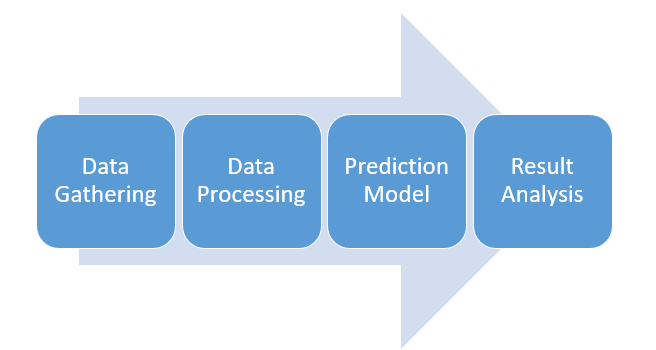
\includegraphics{images/58df7fa7-775c-46ad-92de-4cd885d85079-uscreenshot-439.png}}{}
\makeatother 
\caption{{Sequence Flow of this Report}}
\label{f-f7cf5339f33d}
\end{figure}
\egroup




\subsection{Data \textit{Gathering}}17 years of data of Netflix from March 2002 to March 2019 is used in this prediction model. All the data has been collected from \textbf{https://ftnance.yahoo.com/ }and downloaded under the historical data section. This Historical data is used to predict the future stock prices.



\subsection{Data Processing}



\subsubsection{Data Extraction}The historical data gathered was raw unprocessed data with high volatility. Prediction using this raw data is not a good option so first we need to process this data. Therefore, I have calculated technical indicators. Technical Indicators are the detailed study of past Market action for the purpose of forecasting future prices. It helps in forecasting the price direction and the current trend.
\begin{table}[!htbp]
\caption{{Technical Indicators} }
\label{tw-20db9c32c5c0}
\def\arraystretch{1}
\ignorespaces 
\centering 
\begin{tabulary}{\linewidth}{L}
\hline 
Technical Indicators\\
\tblmidrule 
Simple Moving Average - SMA\\
Exponential Moving Average - EMA\\
Triple Exponential Moving Average - TEMA\\
Kaufman's Adaptive Moving Average - KAMA\\
Moving Average Convergence/Divergence -MACD\\
Bollinger Bands\\
\%B\\
Relative Strength Index - RSI \\
 Average True Range - ATR\\
Chandelier Exit - CE\\
Chande Momentum Oscillator - CMO\\
Force Index - FI\\
Elder-ray\\
Stochastic \%k\\
Stochastic \%D\\
Williams \%R\\
Accumulation Distribution Oscillation - ADO\\
Commodity Channel Index - CCI\\
\tblbottomrule 
\end{tabulary}\par 
\end{table}




\subsubsection{Correlation}After extracting all these features we cannot use all these features in our model the as not all features are relevant some of them are irrelevant and introduces noise in our model. Also, having redundant features confuses our model and therefore increases the computational time. Therefore, we only need to select those features that are related to our stock price, and we could discard other features.

The selection of features was based on the correlation coefficient value of all these features with the original stock's closing prices. The features with the highest correlation value was selected. The correlation techniques used over here where Scatter diagram and Pearson Correlation value.



\paragraph{Scatter Diagram}Scatter diagram is a graph which represents the relation between to data set. In this graph the values of the two data set are plotted along the two axises and the pattern of the resulting graph gives a basic idea about the correlation between the two data set.


\bgroup
\fixFloatSize{images/7c7a74a9-4e3d-4b17-97f3-6b9a6684b180-uscatter-diagram-ma14-days.png}
\begin{figure}[!htbp]
\centering \makeatletter\IfFileExists{images/7c7a74a9-4e3d-4b17-97f3-6b9a6684b180-uscatter-diagram-ma14-days.png}{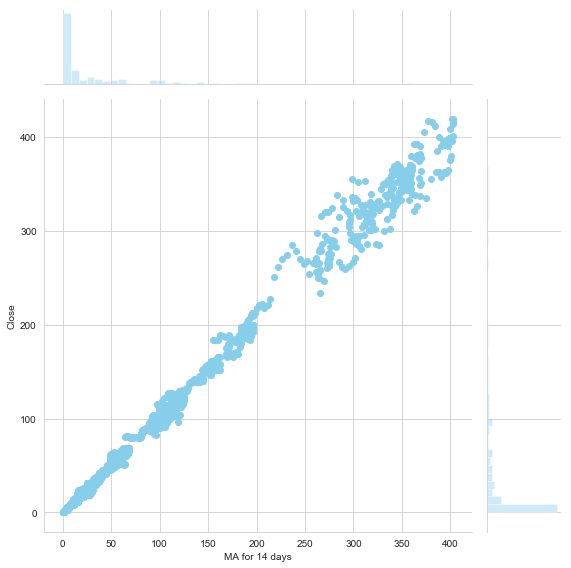
\includegraphics{images/7c7a74a9-4e3d-4b17-97f3-6b9a6684b180-uscatter-diagram-ma14-days.png}}{}
\makeatother 
\caption{{Scatter Diagram for SMA for 14 days vs Close}}
\label{f-fe2e0386c34e}
\end{figure}
\egroup




\paragraph{\textit{Pearson Correlation.}}Pearson Correlation gives a numerical response for finding the relation be- tween different data set. It assigns a number to the extent of relation between two data sets. Its value lies from -1 to 1, 1 representing exactly linear relation between two data sets and 0 representing no relation.

$r\;=\;\frac{\sum_{}((x\;-\;\overline x)(y\;-\;\overline y))}{\sqrt{{\displaystyle\sum_{}}(x\;-\;\overline x)^{2}{\displaystyle\sum_{}}(y\;-\;\overline y)^{2}}}'\;\overline x\;=\;mean\;of\;x $

After analysis the Data using Pearson correlation and verifying using scatter diagram Simple moving average for 14 days was chosen as the parameter for the input for stock prediction for Netflix. A Simple moving average for 14 days of closing price of a stock is defined as the rolling average of closing price of the stocks over the last 14 days. A Simple Moving Average helps in smoothing out the curve which helps in reducing the volatility in the curve.



\subsubsection{Data Transformation}After getting the best feature, the next thing we do is data transformation. Data transformation is used to normalize the data and make the data stationary, which helps in pattern finding. Normalization helps improve convergence of the data. The data was transformed/mapped in the range 0 to 1.

After the data set is transformed into a clean data set, the data set is divided into training and testing sets to evaluate the prediction accuracy of my model. The training set is 95 percent of the total data set and the testing data is the rest of the data.
    
\section{Prediction Model}
After normalizing the data this data was fed into the LSTM network for training. The model was trained for 40 epochs and a batch size of 60. Initially the number of epochs were 100 and changed to find a good prediction model. This LSTM model was initialized of an input sequential layer lead by 4 LSTM layers each having neurons lesser than the previous and then finally a dense output layer with Adam optimizer.


\begin{lstlisting}[style=listing_style,caption={Code for LSTM Neural Network}]
regressor = Sequential() 
regressor.add(LSTM(units = 60, return_sequences = True, input_shape =(X_train.shape [1], 1)))regressor.add(Dropout(0.2)) 
regressor.add(LSTM(units = 45,return_sequences = True)) regressor.add(Dropout(0.2)) 
regressor.add(LSTM(units = 30, return_sequences = True)) 
regressor.add(Dropout(0.2))
regressor.add(LSTM(units = 15))
regressor.add(Dropout(0.2)) 
regressor.add(Dense(units = 1)) 
regressor.compile(optimizer = 'adam', loss = ' mean_squared_error')
regressor.fit(X_train, y_train, epochs = 40, batch_size = 60)
\end{lstlisting}

    
\section{Experimental Result}

\begin{table}[!htbp]
\caption{{Epoch = 40, Feature input = MA14} }
\label{tw-8df77355ef45}
\def\arraystretch{1}
\ignorespaces 
\centering 
\begin{tabulary}{\linewidth}{LLL}
\hline 
Input & RMSE & Size\\
\tblmidrule 
Train &
  2.5983488911838393 &
  3934\\
Test &
  6.39236469202595 &
  223\\
\tblbottomrule 
\end{tabulary}\par 
\end{table}

\bgroup
\fixFloatSize{images/013c96e3-f6d4-433f-9be4-b3eda43dec93-u95-5-ma14-nflx-40-e-train.png}
\begin{figure}[!htbp]
\centering \makeatletter\IfFileExists{images/013c96e3-f6d4-433f-9be4-b3eda43dec93-u95-5-ma14-nflx-40-e-train.png}{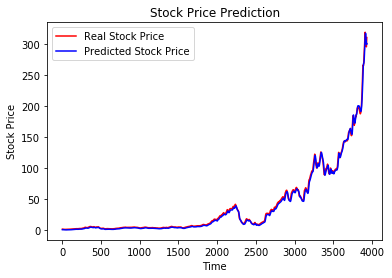
\includegraphics{images/013c96e3-f6d4-433f-9be4-b3eda43dec93-u95-5-ma14-nflx-40-e-train.png}}{}
\makeatother 
\caption{{Result of LSTM model for Train data set}}
\label{f-dd2f0d7b37b6}
\end{figure}
\egroup

\bgroup
\fixFloatSize{images/164fee09-21a5-4e60-abf9-e220aadfb1e7-u95-5-ma14-nflx-40-e.png}
\begin{figure}[!htbp]
\centering \makeatletter\IfFileExists{images/164fee09-21a5-4e60-abf9-e220aadfb1e7-u95-5-ma14-nflx-40-e.png}{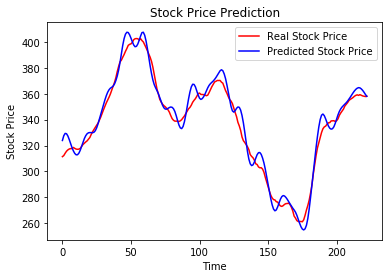
\includegraphics{images/164fee09-21a5-4e60-abf9-e220aadfb1e7-u95-5-ma14-nflx-40-e.png}}{}
\makeatother 
\caption{{Result of LSTM model for Test data set}}
\label{f-546de945d1f7}
\end{figure}
\egroup
After performing continuous simulations for different number of features and epochs, we have observed that by  taking MA14 feature with 40 epochs we are able to achieve  nearly the best results with training RMSE of \textbf{2.5983488911838393 } and testing RMSE of \textbf{6.39236469202595.}
    
\section{Conclusion}
In this work, I tried to predict the future stock price using LSTM. Simple moving average for 14 days was used as an input parameter of a 60-day sliding window approach. I would like to highlight forecasting stock prices are very much helpful for investors to earn huge profit. Predicting future price of a given stock to produce an accurate result is encouraging researchers to find some new technique to improve the accuracy. RNNs like LSTM are very good at processing sequential time series data. LSTM has been proven a very good solution while dealing with sequential data streams. In this work, I was able to produce significantly good result using a sliding window approach and LSTM model to predict the future price of Netflix stocks. 
    
\section{List of abbreviations}

    



\bibliographystyle{elsarticle-num}

\bibliography{\jobname}

\end{document}
